\mainmatter%
\setcounter{page}{1}

\lectureseries[\course]{\course}

\auth[\lecAuth]{Lecturer: \lecAuth\\ Scribe: \scribe}
\date{November 24, 2009}

\setaddress%

% the following hack starts the lecture numbering at 16
\setcounter{lecture}{15}
\setcounter{chapter}{15}

\lecture{Viscosity Solutions}

\section{Exit Problem}
Last time we had the exit problem where
\begin{align*}
0 = \rho - |\nw(x)|^2, &\qquad |x|<R \\
W(x) = 0, &\qquad |x|=R
\end{align*}

In this lecture we will go to the one dimensional case and find a viscosity solution for the exit problem.
We start with
\begin{align}
\label{eq:16exit}
&0 = 1-{(W_x)}^2~\forall x\in G=(-1,1) \\
\label{eq:16exittc}
&W(-1) = W(1) = 0
\end{align}
(\ref{eq:16exit}) implies $W_x(x)=\pm1~\forall x$ which also implies that there does not exist a classical solution for (\ref{eq:16exit}) and (\ref{eq:16exittc}).

Note that a weak solution requires that (\ref{eq:16exit}) is satisfied A.E. (almost everywhere).
It is sufficient to satisfy (\ref{eq:16exit}) except on a finite (or countably infinite) set of points.
Examples of weak solutions are (see Figure~\ref{fig:16w})
\begin{align*}
W^1(x) &= |x|-1 \\
W^2(x) &= 1-|x| \\
W^3(x) &= \ldots
\end{align*}
There are an infinite number of weak solutions that satisfy (\ref{eq:16exit}) and (\ref{eq:16exittc}) but we only want one of them.

\begin{figure}[ht!]
\centering
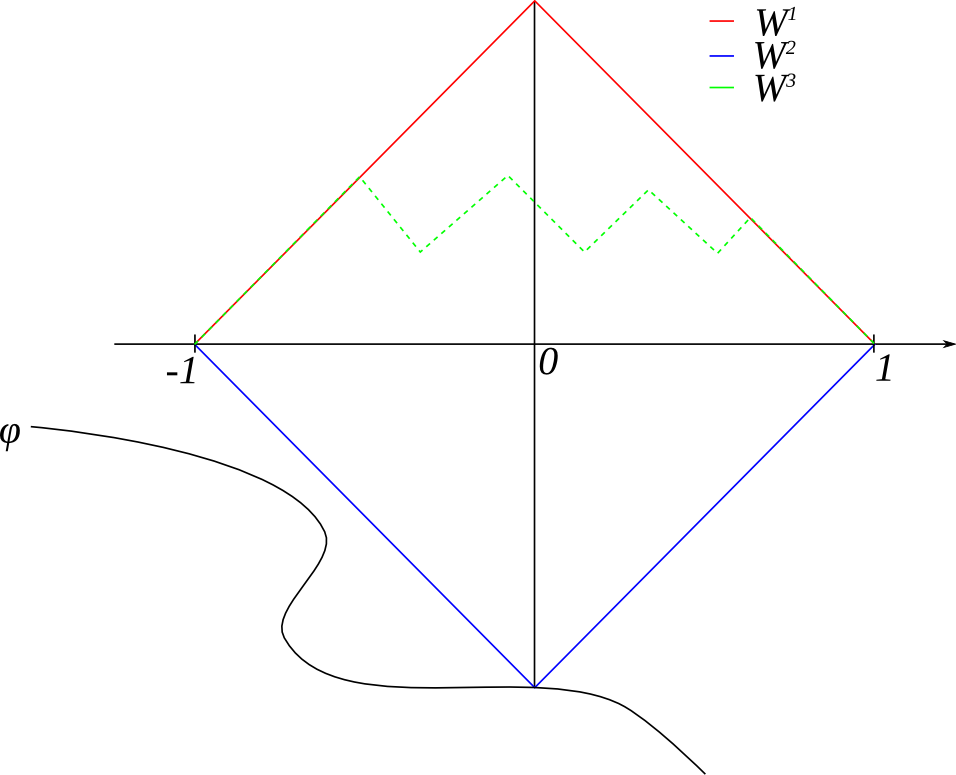
\includegraphics[width=.4\textwidth]{images/16w}
\caption{Possible solutions using classical methods.}
\label{fig:16w}
\end{figure}

\section{Viscosity Solutions}
Typically there exists a viscosity solution to the HJB and HJI PDE problems.
Recall that HJB is for control problems and HJI is for game theory problems.
For a solution to be a viscosity solution it must satisfy
\begin{align}
\label{eq:16vsf}
0 = F(x,\nw(x))~\forall x\in G
\end{align}

\begin{definition}
$W\in C(G)$ is a \textit{viscosity subsolution} at $x_0\in G$ if given any $\vp\in C^1(G)$ s.t. $W(x)-\vp(x)$ is a local minimum at $x_0$, we have
$$F(x_0,\nabla\vp(x_0))\leq0$$
\end{definition}

\begin{definition}
$W\in C(G)$ is a \textit{viscosity supersolution} at $x_0\in G$ if given $\vp\in C^1(G)$ s.t. $W(x)-\vp(x)$ has a local maximum at $x_0$, we have
$$F(x_0,\nabla\vp(x_0))\geq0$$
\end{definition}

\begin{definition}
$W\in C(G)$ is a \textit{viscosity solution} if it is both a viscosity subsolution and a viscosity supersolution at $x_0$.
\end{definition}

\begin{definition}
$W$ is a viscosity solution on $G$ if it is a viscosity solution $\forall x_0\in G$.
\end{definition}

\begin{remark}
We might as well require $W(x_0)=\vp(x_0)$ in the definition since there is no zeroth-order term in (\ref{eq:16vsf}).
\end{remark}

\begin{remark}
Suppose $W$ is a classical solution at $x_0$ such that
$$W\in C^1(R_\delta(x_0)), F(x_0,\nw(x_0))=0$$
Further, suppose that $\vp\in C^1$ and $W-\vp$ is a local minimum at $x_0$.
Then
\begin{itemize}
\item $0 = \nabla[W-\vp](x_0) = \nabla W(x_0)-\nabla\vp(x_0)$
\item $0 = F(x_0,\nabla u(x_0)) = F(x_0,\nabla\vp(x_0))$
\item The viscosity subsolution conditions are satisfied.
      Similarly, the viscosity supersolution conditions are satisfied.
      Therefore $W$ is a viscosity solution at $x_0$.
\item Any classical solution is a viscosity solution! See Figure~\ref{fig:16x0}.
\end{itemize}
\end{remark}

\begin{figure}[ht!]
\centering
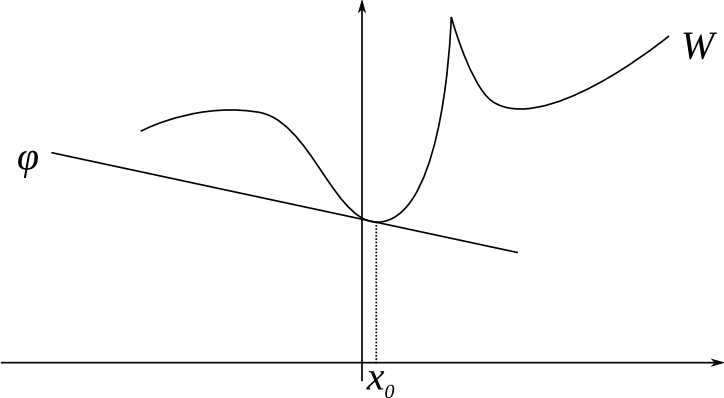
\includegraphics[width=.4\textwidth]{images/16x0}% chktex 29
\caption{Gradient at $x_0$.}
\label{fig:16x0}
\end{figure}

\begin{example}
We start by examining (\ref{eq:16exit}) for $W^1$.
We have that
$$W^1\in C^1(\mathcal{A}), \mathcal{A}=(-1,0)\cup(0,1)$$
satisfies (\ref{eq:16exit}) on $\mathcal{A}$ so $W^1$ is a viscosity solution on $\mathcal{A}$.
However, we still need to check $x_0=0$.

Suppose that $\vp\in C^1(G)$ and $W-\vp$ has a local maximum at $x_0=0$.
This is not possible (see Figure~\ref{fig:16w} where it can be seen that $W^1$ only has a local minimum at $x_0=0$).
By default $W^1$ is a viscosity supersolution.

\begin{figure}[ht!]
\centering
\includegraphics[width=.4\textwidth]{images/16vs}
\caption{Convexity of $W$ means no viscosity solution.}
\label{fig:16vs}
\end{figure}

Now, suppose that $\vp\in C^1(G)$ and $W-\vp$ has a local minimum at $x_0=0$.
Then let $\vp(x)\equiv-1$.
This shows that conditions (\ref{eq:16exit}) and (\ref{eq:16exittc}) are satisfied.
But, we see that
$$F(0,\vp_x(0))=1-0^2=1>0$$
therefore $W^1$ is not a viscosity subsolution and hence $W^1$ is not a viscosity solution.

This result can be generalized more than that though.
Suppose that $W$ has a convex corner as in Figure~\ref{fig:16vs}, then $W$ is not a viscosity solution.

Next, we will look at $W^2$.
Clearly this is a solution for all $x\in\mathcal{A}$.
Checking $x_0=0$ shows that there does not exist $\vp\in C^1(G)$ such that $W-\vp$ has a local minimum at $x_0=0$ because there is no $\vp$ that exists so we don't have to check $F(x_0,\nabla\vp(x_0))$, therefore $W^2$ is a viscosity subsolution.

Now, let $\vp\in C^1(G)$.
Then $W^2-\vp$ has a local maximum at $x_0=0$ and $\vp_x(0)\in[-1,1]$
\begin{align*}
&\therefore F(0,\vp_x(0)) = 1-{(\vp_x(0))}^2\geq0
\end{align*}
Therefore, $W^2$ is a viscosity solution.
$\lozenge$
\end{example}

\begin{figure}[ht!]
\centering
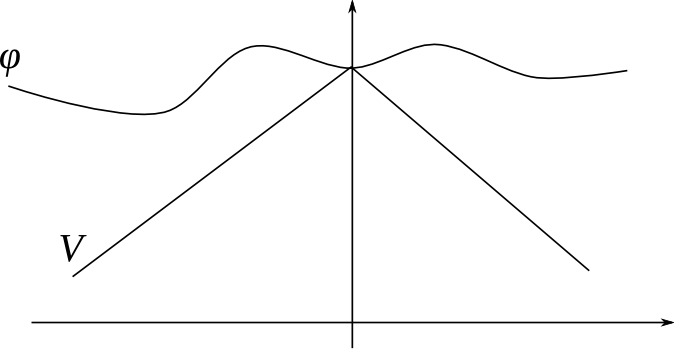
\includegraphics[width=.4\textwidth]{images/16subsol}
\caption{Viscosity subsolution.}
\label{fig:16subsol}
\end{figure}

\section{Finite Time Horizon Deterministic Control}
Let the system dynamics and initial conditions be
\begin{align*}
\dot{\xi} = f(\xi,u), \qquad \xi_s=x\in\mathbb{R}^n
\end{align*}
The cost function is
$$J(s,x;u.) = \int_s^t l(\xi_t,u_t)dt+\psi(\xi_T)$$
and the value function is
$$V(s,x) = \inf_{\uinu_s}J(s,x;u.)$$
The DPP is
$$V(s,x) = \inf_{\uinu_x}\left\lbrace \int_s^t l(\xi_t,u_t)dt+V(t,\xi_t) \right\rbrace$$
and the DPE/HJB PDE is
\begin{align}
\label{eq:16dpe}
&0 = V_s + \inf_{v\in\mathcal{U}}\left\lbrace l(x,v)+f(x,v)\cdot\nabla_x V\right\rbrace \\
&V(T,x) = \psi(x) \nonumber
\end{align}

We want to show that the viscosity solution is the value function.

Suppose that
\begin{align}
\label{eq:16vp}
\begin{split}
&\vp(s,x)=V(s,x) \\
&\vp(t,y)\geq V(t,y)~\forall t,y \\
&\vp\in C^1(0,T)\times\mathbb{R}^n
\end{split}
\end{align}
Next, the Fundamental Theorem of Calculus shows that, for any $\uinu_s$, we have
\begin{align}
\label{eq:16fund}
\vp(t,\xi_t)-\vp(s,x) = \int_s^t\vp_s(r,\xi_r)+\nabla_x\vp(r,\xi_r)\cdot f(\xi_r,u_r)dr
\end{align}

(\ref{eq:16vp}) implies
\begin{align}
\label{eq:16vpv}
\vp(t,\xi_t)-\vp(s,x)\geq V(t,\xi_t)-V(s,x)
\end{align}

Now, suppose that $l$ and $f$ are in $C^1$, are globally bounded and are Lipschitz smooth.
Also, suppose there exists an optimal $\bar{u}$ in the HJB PDE, i.e.,
\begin{align}
\label{eq:16ubar}
l(x,\bar{u})+f(x,\bar{u})\cdot\nabla_x\vp(s,x) = \inf_{v\in\mathcal{U}}\left\lbrace l(x,v)+f(x,v)\cdot\nabla_x\vp(s,x)\right\rbrace
\end{align}
Let $u_t^\ast=\bar{u}$.
By (\ref{eq:16dpe}) we have
$$V(s,x)\leq\int_s^t l(\xi_t^\ast,u_t^\ast)dt+V(t,\xi_t^\ast)$$
which can be re-written as
\begin{align}
\label{eq:16v}
V(s,x)-V(t,\xi_t^\ast)\leq\int_s^t l(\xi_t^\ast,\bar{u})dt
\end{align}
By (\ref{eq:16vpv}) and (\ref{eq:16v}) we get
$$\vp(s,x)-\vp(t,\xi_t^\ast) = \int_s^t l(\xi_t^\ast,\bar{u})dt$$
This can be expanded to show
\begin{align*}
\underbrace{\vp(s,x) - \vp(t,\xi_t^\ast)}_{\lambda} &\leq \int_s^t l(\xi_r^\ast,\bar{u}) + \vp_s(r,\xi_r^\ast) + \nabla_x\vp(r,\xi_r^\ast)\cdot f(\xi_r^\ast,\bar{u})dr \\
&\qquad - \underbrace{\int_s^t\vp_r(r,\xi_r^\ast) + \nabla_x\vp(r,\xi_r^\ast)\cdot f(\xi_r^\ast,\bar{u})dr}_{\lambda}
\end{align*}
Then, by (\ref{eq:16fund}) we have $\lambda=\lambda$ and this leads to
$$0\leq\int_s^t l(\xi_r^\ast,\bar{u}) + \vp_s(r,\xi_r^\ast) + \nabla_x\vp(r,\xi_r^\ast)\cdot f(\xi_r^\ast,\bar{u})dr$$
Note that, from Gr\"onwall's inequality to show boundedness, we also have
\begin{align*}
\xi_t^\ast-x &= \int_s^t f(\xi_r^\ast,\bar{u})dr \\
\Rightarrow |\xi_t^\ast-x| &\leq \int_s^t|f(x,\bar{u})|dr + \int_s^t|f(\xi_r^\ast,\bar{u})-f(x,\bar{u})|dr \\
&\leq M(t,s)-\int_s^t K|\xi_r^\ast-x|dr \\
\Rightarrow |\xi_t^\ast-x| &\leq M(t-s) + \int_s^t M(r-s)Ke^{K(t-s)}dr
\end{align*}
If $t-s<\delta$ then we get
$$|\xi_t^\ast-x|\leq C(t-s)$$
This leads to
\begin{align*}
&|l(\xi_r^\ast,\bar{u}) - l(x,\bar{u})| \leq K_l|\xi_r^\ast-x| \leq K_l C(r-s) \\
\Rightarrow &0 \leq \int_s^{s+\delta}l(x,\bar{u})+\vp_r(x,\bar{u})+\nabla_x\vp(s,x)\cdot f(x,\bar{u})dr + \mathcal{O}(\delta^2)
\end{align*}
Then,
\begin{align*}
&0 \leq \delta\left[ l(x,\bar{u})+\vp_s(s,x)+\nabla_x\vp(s,x)\cdot f(x,\bar{u})\right] + \mathcal{O}(\delta^2) \\
\Rightarrow &l(x,\bar{u}) + \vp_s(s,x) + \nabla_x\vp(s,x)\cdot f(x,\bar{u}) \geq 0 \\
&0 \leq \vp_s(s,x) + \inf_{v\in\mathcal{U}}\left\lbrace l(x,v) + \nabla_x\vp(s,x)\cdot f(x,v)\right\rbrace \\
\end{align*}
and therefore $V$, the value function, is a viscosity solution.

\section{Numerical Methods for Viscosity Solutions}
We will go back to the exit problem where
\begin{align*}
&0 = \inf_{v\in\mathcal{U}}\left\lbrace f(x,v)\cdot\nabla_x W(x)+l(x,v)\right\rbrace, \qquad x\in G \\
&W(x) = \psi(x), \qquad x\in\partial G
\end{align*}
The DPP is
$$V(x) = \inf_{\uinu}\left\lbrace \int_0^{t\wedge\tau}l(\xi_r,u_r)dr + I_{t\leq\tau}V(\xi_t) + I_{t\geq\tau}\psi(\xi_t)\right\rbrace$$
Here we have introduced the notation $t\wedge\tau$ which means $\min\{t,\tau\}$ and $I_{t\leq\tau}$ which means to use the expression following the $I$ operator if the subscript is true or to move on to the next $I$ operator if the subscript is false.

Let $x_{i,j}$ be an interior point on $G$ (see Figures~\ref{fig:16grid} and~\ref{fig:16x}) and let $h=t\ll 1$ such that $h<\tau(x_{i,j},u)$ for all $\epsilon$-optimal $u$ so that we cannot exit the interior of $G$ in one time step.
Then, the value function is
$$V(x_{i,j}) = \inf_u\left\lbrace \int_0^h l(\xi_t,u_t)dt+V(\xi_h)\right\rbrace$$
We iterate $V^k$ on the grid points as seen in Figure~\ref{fig:16grid}.
Let the iteration follow
$$V^{k+1}(x_{i,j}) = \inf_u\left\lbrace \int_0^h l(\xi_t,u_t)dt + V^k(\xi_t)\right\rbrace$$
Suppose $h\ll 1$ such that $\xi_h\in\mathcal{S}$ and linearize and we get
$$V^{k+1}(x_{i,j}) = \inf_u\left\lbrace \int_0^h l(x_{i,j},u)dr+V^k(x_{i,j}+hf(x_{i,j},u))\right\rbrace$$

\begin{figure}[ht!]
\centering
\includegraphics[width=.4\textwidth]{images/16grid}
\caption{Grid for the space $G$.}
\label{fig:16grid}
\end{figure}

\begin{figure}[ht!]
\centering
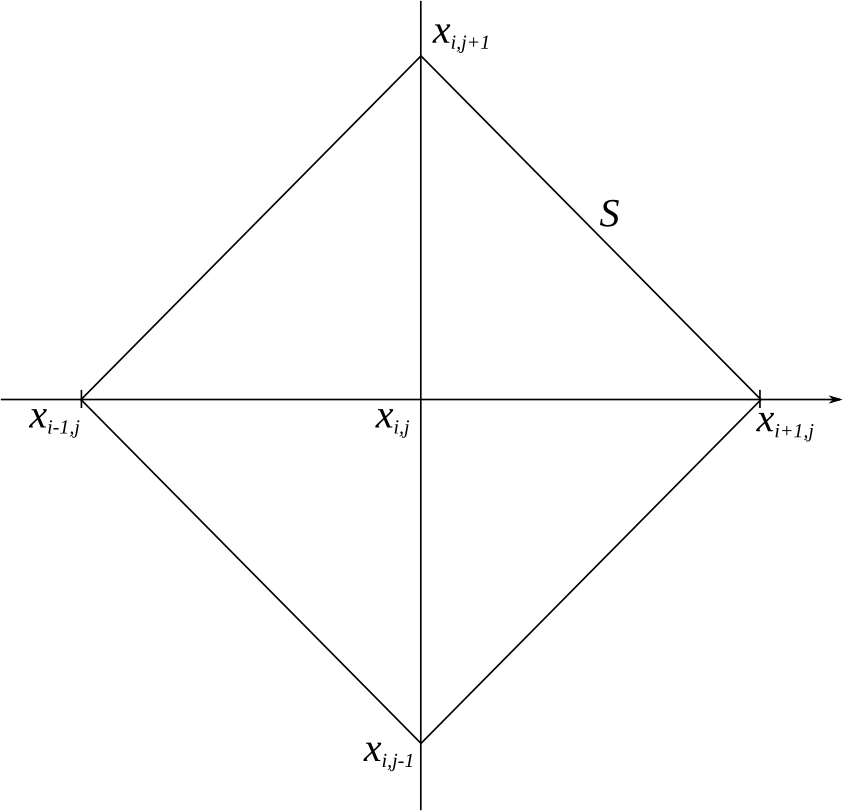
\includegraphics[width=.4\textwidth]{images/16x}
\caption{Zoomed in area around the point $x_{ij}$.}
\label{fig:16x}
\end{figure}

Note that we will continue this topic in the next lecture.% chktex 17
